\documentclass{article}

% Add necessary packages
\usepackage{natbib, graphicx, fancyhdr} % For managing references
% natbib for bibtext

% Add necessary commands
\bibliographystyle{plainnat} % Specify the bibliography style

% Define margins
\setlength{\topmargin}{-1.0cm}
\setlength{\oddsidemargin}{0.1cm}
\setlength{\textwidth}{16.5cm}
\setlength{\textheight}{23.0cm}

\graphicspath{{images/}} %configuring the graphicx package

% Define header and footer
\pagestyle{fancy}
\fancyhf{}
\lhead{{
\includegraphics[height=.65cm]{etsiit-1.png}}}
\rhead{\textbf{\textit{First Formal Progress Review}} }
\cfoot{\textbf{\textit{\thepage}}}
% \lfoot{\textbf{\textit{Page \thepage/\pageref*{LastPage}}}}
% \rfoot{\textbf{\textit{Alejandro Romero Prieto}}}
% \renewcommand{\footrulewidth}{0.7pt}
\renewcommand{\headrulewidth}{0.7pt}
\setlength{\headheight}{23pt}

% This is to define a style with no footer for the table of contents
\fancypagestyle{nofooter}{%
	\fancyfoot{}%
}




% Add necessary packages

% Add necessary commands
\bibliographystyle{plainnat} % Specify the bibliography style


% Define margins
\setlength{\topmargin}{-1.0cm}
\setlength{\oddsidemargin}{0.1cm}
\setlength{\textwidth}{16.5cm}
\setlength{\textheight}{23.0cm}

\graphicspath{{images/}} %configuring the graphicx package

% Define header and footer
\pagestyle{fancy}
\fancyhf{}
\lhead{{
\includegraphics[height=.65cm]{etsiit-1.png}}}
\rhead{\textbf{\textit{Práctica 6: Laboratorio}} }
\cfoot{\textbf{\textit{\thepage}}}
% \lfoot{\textbf{\textit{Page \thepage/\pageref*{LastPage}}}}
% \rfoot{\textbf{\textit{Alejandro Romero Prieto}}}
% \renewcommand{\footrulewidth}{0.7pt}
\renewcommand{\headrulewidth}{0.7pt}
\setlength{\headheight}{23pt}

% This is to define a style with no footer for the table of contents
\fancypagestyle{nofooter}{%
  \fancyfoot{}%
}



% Title Page %%%%%%%%%%%%%%%%%%%%%%%%%%%%%%%%%%%%%%%%%%%%%%%%%%%%%%%%%%%%%%%%%%%%%%%%%%%%%%%% 

\begin{document}
\begin{center}
  \vspace*{0.5\baselineskip} % Reduced space
  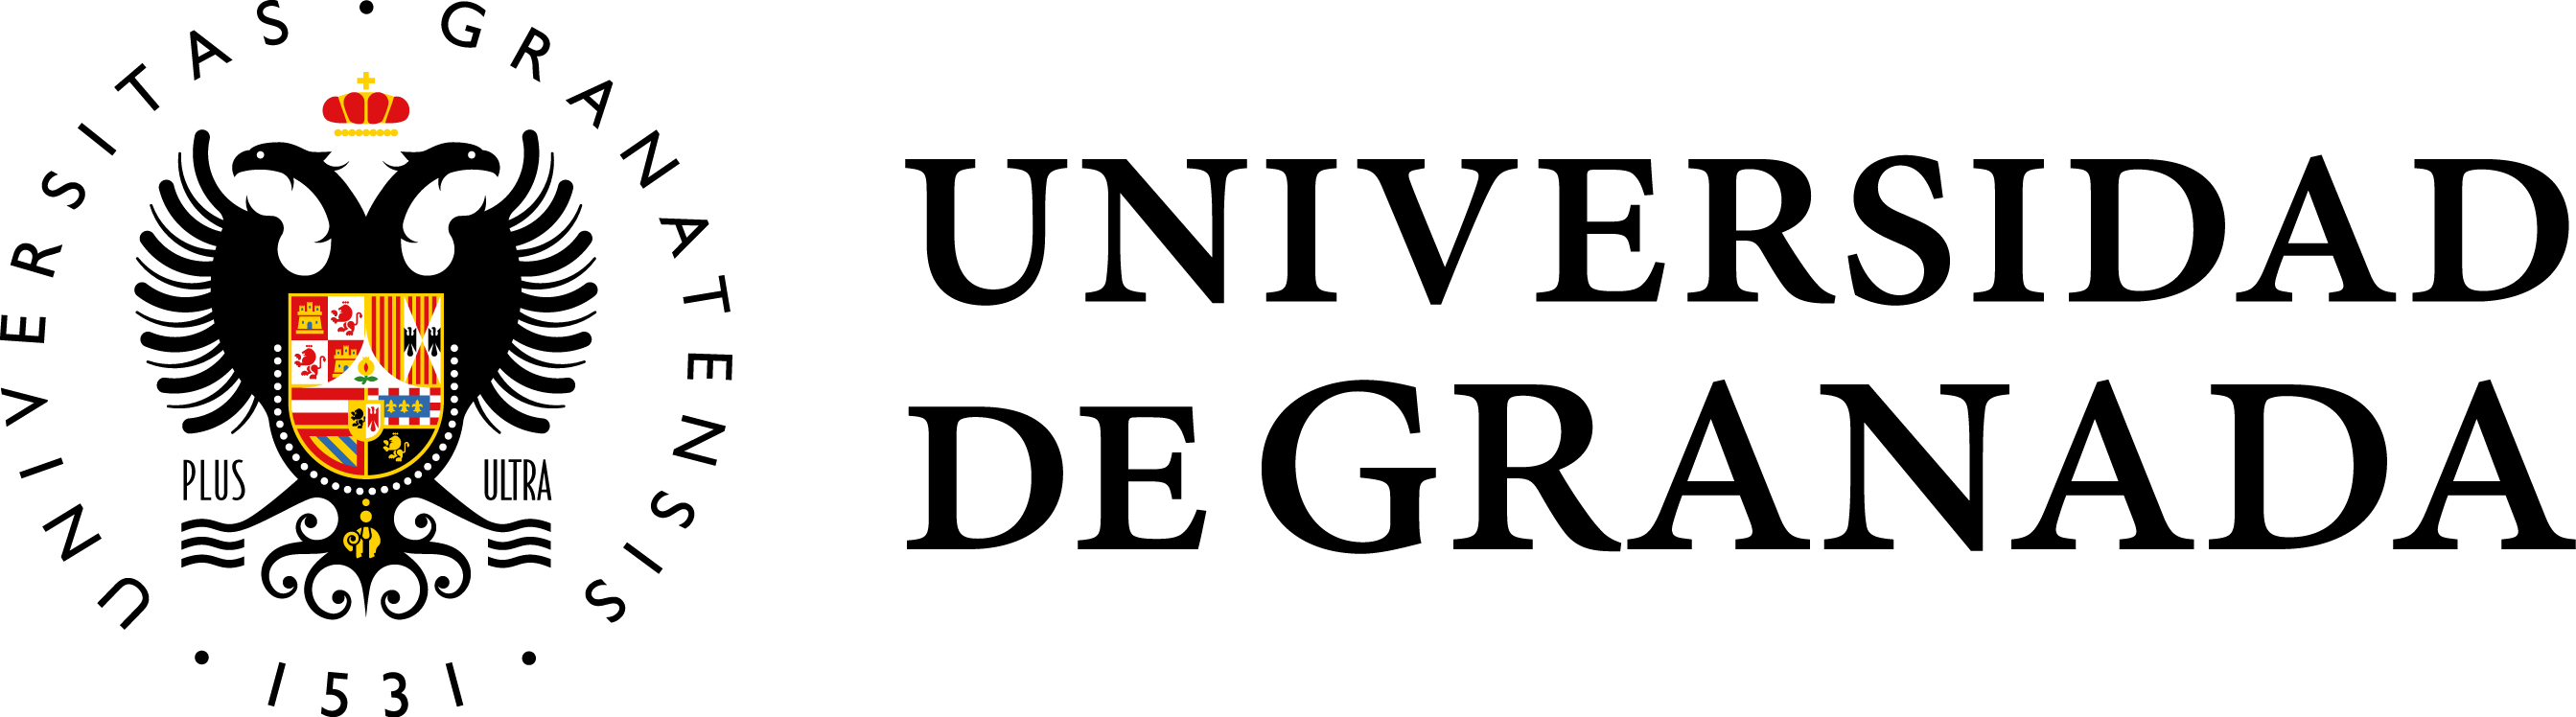
\includegraphics[width=0.8\textwidth]{ugr-2.png}\\
  \vfill
  %\vspace*{8\baselineskip} % Reduced space
  {\Huge \textbf{Laboratorio}}\\ % Enlarged font
  \vspace*{2\baselineskip}
  {\LARGE \textbf{Practica 6 Ingeniería Gráfica}}\\
  \begin{large}
    \vspace*{1\baselineskip}
    {\Large Torres Ramos, Juan Luis \\}
	\vspace*{0.5\baselineskip}
    {{ g20596044@correo.ugr.es}}\\[1cm]
    %\vspace*{4\baselineskip}
    \vfill
	{Universidad de Granada}\\
    {\large ETSIIT}\par
	{\large 12/12/2024}\par
	\vspace*{3\baselineskip}
  \end{large}
  \thispagestyle{empty} 
\end{center}
\pagebreak





% Contents %%%%%%%%%%%%%%%%%%%%%%%%%%%%%%%%%%%%%%%%%%%%%%%%%%%%%%%%%%%%%%%%%%%%%%%%%%%%%%%%%%%%%%%%

% \lhead{\emph{Contents}} % Set the left side page header to "Contents"
%\tableofcontents
%	\thispagestyle{nofooter}
%	%\include{abstract/abstract}
%	\cleardoublepage
%	\typeout{}

%\pagebreak

% Student %%%%%%%%%%%%%%%%%%%%%%%%%%%%%%%%%%%%%%%%%%%%%%%%%%%%%%%%%%%%%%%%%%%%%%%%%%%%%%%%%%%%%%%%%

\setcounter{page}{1}

\section*{Práctica 6 Final: Laboratorio}

Para ejecutar el proyecto, simplemente ejecute el comando `make total` en la terminal. Esto compilará todos los archivos necesarios y generará el documento final.

\subsection*{Primera Escena: Interacción con una Máquina Analizadora de Manzanas}

\begin{enumerate}
    \item \textbf{Selección Interactiva} \\
    Se implementó un sistema de botones interactivos, cada uno con animaciones propias. Interactuas con ellos con el boton del medio. 

    \item \textbf{Control de Iluminación} \\
    Desde el panel de control, el botón amarillo permite encender y apagar las luces de forma.

    \item \textbf{Primera Escena: Análisis de la Manzana} \\
    En la primera escena, una máquina analiza una manzana mediante el panel de control. Tiene un cristal, un material que añado como "extra". Con el botón rojo del panel se puede experimentar con diferentes visualizaciones y texturas:
    \begin{itemize}
        \item Dibujado Flat: Representación plana de la superficie.
        \item Dibujado Smooth: Representación suave de las formas.
        \item Manzana de Oro: Aplicación de textura dorada.
        \item Visión en Líneas: Representación de líneas del modelo.
        \item Textura de Mármol: Texturizado automático lineal de OpenGL.
        \item Textura de Madera: Texturizado cilíndricas.
        \item Textura de Metal: Texturizado esférico
        \item Transformación a Dado: Convierte la manzana en un dado. Texturizado de Coordenadas Manual. 
    \end{itemize}

    \item \textbf{Cambio de Escena} \\
    El botón azul en el panel de control permite avanzar a la segunda escena.
\end{enumerate}

\begin{figure}[h]
\centering
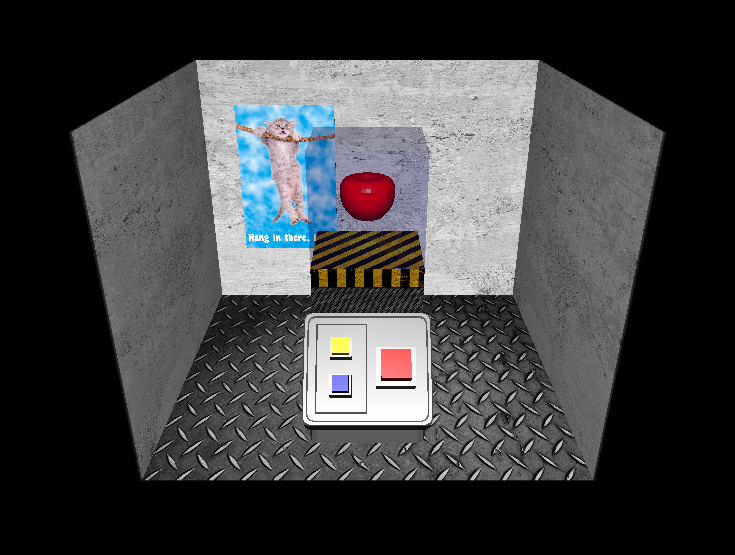
\includegraphics[width=0.6\textwidth]{./images/Escena1.png}
\caption{Escena 1}
\end{figure}	


\pagebreak
\subsection*{Segunda Escena: Brazo Mecánico y Hombre Lobo}

\begin{itemize}
    \item \textbf{Brazo Mecánico} \\
    Con el botón rojo se activa una animación predeterminada del brazo mecánico. Además, es posible controlar manualmente sus 9 ejes mediante el teclado:
    \begin{itemize}
        \item Teclas: q, w, e, r, t, y, u, a (esta última mueve 2 ejes simultáneamente).
        \item Uso de mayúsculas para mover en una dirección y minúsculas para la dirección opuesta.
    \end{itemize}

    \item \textbf{Hombre Lobo y Efectos Especiales} \\
    El escenario incluye un estante con un modelo de un hombre lobo que tiene una textura segun las coordenadas de textura de dicho modelo. Como detalle adicional, al presionar el botón morado ubicado en el estante, se activa un efecto especial de "discoteca".
\end{itemize}

\begin{figure}[h]
	\centering
	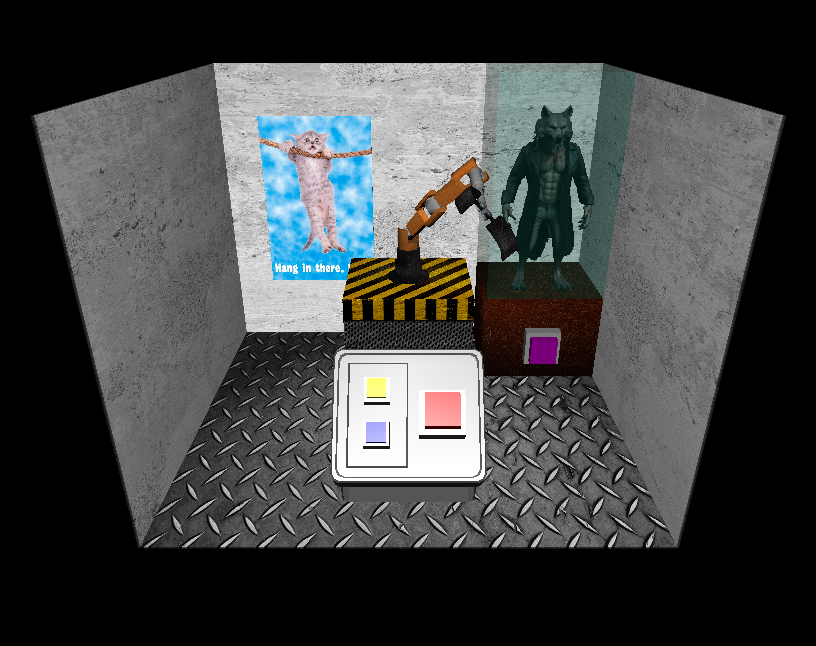
\includegraphics[width=0.6\textwidth]{./images/Escena2.png}
	\caption{Escena 2}
	\end{figure}	

\end{document}